\begin{flushright} {\tiny {\color{gray} (tikz\_staggered2D\_4x3.tex)}} \end{flushright}
%~~~~~~~~~~~~~~~~~~~~~~~~~~~~~~~~~~~~~~~~~~~~~~~~~~~~~~~~~~~~~~~~~~~~~~~~~~~~~~~~~~~~~~~~~~~~~~~~~~


\begin{center}
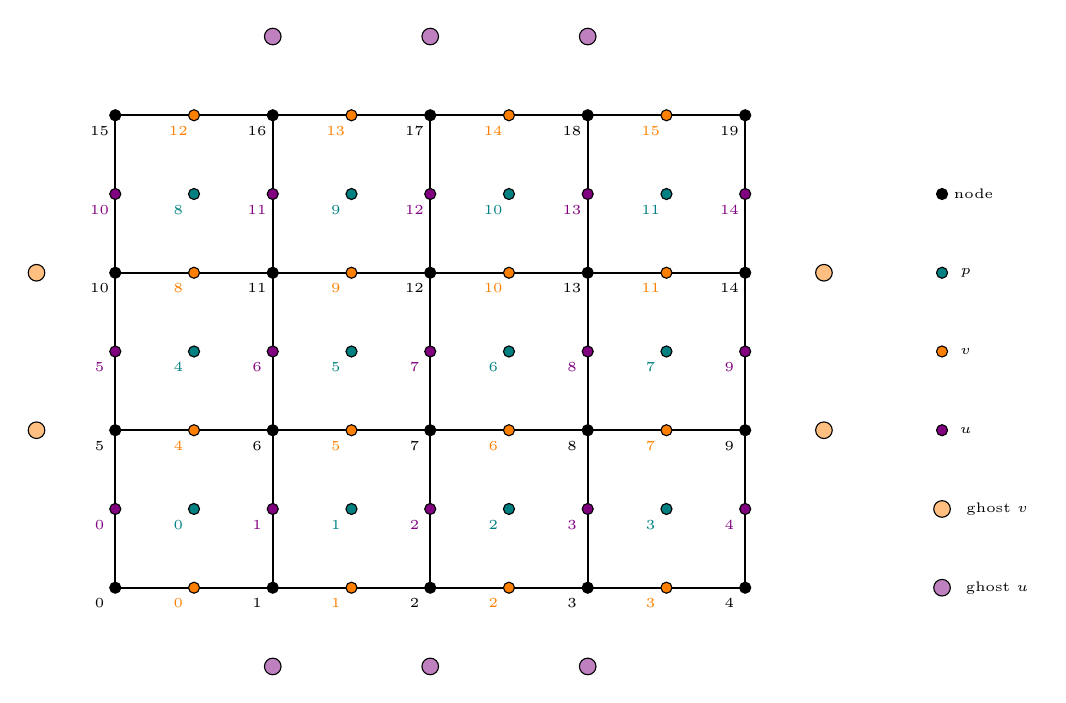
\begin{tikzpicture}
%\draw[fill=gray!23,gray!23](0,0) rectangle (12,10);
%\draw[step=0.5cm,gray,very thin] (0,0) grid (12,10); %background grid

\draw[thick] (0,0) -- (8,0) -- (8,6) -- (0,6) -- cycle ; %1-4
\draw[thick] (0,2) -- (8,2)  ; 
\draw[thick] (0,4) -- (8,4)  ; 
\draw[thick] (2,0) -- (2,6)  ; 
\draw[thick] (4,0) -- (4,6)  ; 
\draw[thick] (6,0) -- (6,6)  ; 

%pressure nodes
\draw[black,fill=teal] (1,1)   circle (2pt); 
\draw[black,fill=teal] (3,1)   circle (2pt); 
\draw[black,fill=teal] (5,1)   circle (2pt); 
\draw[black,fill=teal] (7,1)   circle (2pt); 

\draw[black,fill=teal] (1,3)   circle (2pt); 
\draw[black,fill=teal] (3,3)   circle (2pt); 
\draw[black,fill=teal] (5,3)   circle (2pt); 
\draw[black,fill=teal] (7,3)   circle (2pt); 

\draw[black,fill=teal] (1,5)   circle (2pt); 
\draw[black,fill=teal] (3,5)   circle (2pt); 
\draw[black,fill=teal] (5,5)   circle (2pt); 
\draw[black,fill=teal] (7,5)   circle (2pt); 

\node[] at (0.8,0.8) {\tiny \color{teal} 0};
\node[] at (2.8,0.8) {\tiny \color{teal} 1};
\node[] at (4.8,0.8) {\tiny \color{teal} 2};
\node[] at (6.8,0.8) {\tiny \color{teal} 3};

\node[] at (0.8,2.8) {\tiny \color{teal} 4};
\node[] at (2.8,2.8) {\tiny \color{teal} 5};
\node[] at (4.8,2.8) {\tiny \color{teal} 6};
\node[] at (6.8,2.8) {\tiny \color{teal} 7};

\node[] at (0.8,4.8) {\tiny \color{teal} 8};
\node[] at (2.8,4.8) {\tiny \color{teal} 9};
\node[] at (4.8,4.8) {\tiny \color{teal} 10};
\node[] at (6.8,4.8) {\tiny \color{teal} 11};

% u nodes
\draw[black,fill=violet] (0,1)   circle (2pt); 
\draw[black,fill=violet] (2,1)   circle (2pt); 
\draw[black,fill=violet] (4,1)   circle (2pt); 
\draw[black,fill=violet] (6,1)   circle (2pt); 
\draw[black,fill=violet] (8,1)   circle (2pt); 

\draw[black,fill=violet] (0,3)   circle (2pt); 
\draw[black,fill=violet] (2,3)   circle (2pt); 
\draw[black,fill=violet] (4,3)   circle (2pt); 
\draw[black,fill=violet] (6,3)   circle (2pt);
\draw[black,fill=violet] (8,3)   circle (2pt);

\draw[black,fill=violet] (0,5)   circle (2pt); 
\draw[black,fill=violet] (2,5)   circle (2pt); 
\draw[black,fill=violet] (4,5)   circle (2pt); 
\draw[black,fill=violet] (6,5)   circle (2pt);
\draw[black,fill=violet] (8,5)   circle (2pt);

\node[] at (-0.2,0.8) {\tiny \color{violet} 0};
\node[] at (1.8,0.8)  {\tiny \color{violet} 1};
\node[] at (3.8,0.8)  {\tiny \color{violet} 2};
\node[] at (5.8,0.8)  {\tiny \color{violet} 3};
\node[] at (7.8,0.8)  {\tiny \color{violet} 4};

\node[] at (-0.2,2.8) {\tiny \color{violet} 5};
\node[] at (1.8,2.8)  {\tiny \color{violet} 6};
\node[] at (3.8,2.8)  {\tiny \color{violet} 7};
\node[] at (5.8,2.8)  {\tiny \color{violet} 8};
\node[] at (7.8,2.8)  {\tiny \color{violet} 9};

\node[] at (-0.2,4.8){\tiny \color{violet} 10};
\node[] at (1.8,4.8) {\tiny \color{violet} 11};
\node[] at (3.8,4.8) {\tiny \color{violet} 12};
\node[] at (5.8,4.8) {\tiny \color{violet} 13};
\node[] at (7.8,4.8) {\tiny \color{violet} 14};

% v nodes
\draw[black,fill=orange] (1,0)   circle (2pt); 
\draw[black,fill=orange] (3,0)   circle (2pt); 
\draw[black,fill=orange] (5,0)   circle (2pt); 
\draw[black,fill=orange] (7,0)   circle (2pt); 

\draw[black,fill=orange] (1,2)   circle (2pt); 
\draw[black,fill=orange] (3,2)   circle (2pt); 
\draw[black,fill=orange] (5,2)   circle (2pt); 
\draw[black,fill=orange] (7,2)   circle (2pt); 

\draw[black,fill=orange] (1,4)   circle (2pt); 
\draw[black,fill=orange] (3,4)   circle (2pt); 
\draw[black,fill=orange] (5,4)   circle (2pt); 
\draw[black,fill=orange] (7,4)   circle (2pt); 

\draw[black,fill=orange] (1,6)   circle (2pt); 
\draw[black,fill=orange] (3,6)   circle (2pt); 
\draw[black,fill=orange] (5,6)   circle (2pt); 
\draw[black,fill=orange] (7,6)   circle (2pt); 

\node[] at (0.8,-0.2) {\tiny \color{orange} 0};
\node[] at (2.8,-0.2) {\tiny \color{orange} 1};
\node[] at (4.8,-0.2) {\tiny \color{orange} 2};
\node[] at (6.8,-0.2) {\tiny \color{orange} 3};

\node[] at (0.8,1.8) {\tiny \color{orange} 4};
\node[] at (2.8,1.8) {\tiny \color{orange} 5};
\node[] at (4.8,1.8) {\tiny \color{orange} 6};
\node[] at (6.8,1.8) {\tiny \color{orange} 7};

\node[] at (0.8,3.8) {\tiny \color{orange} 8};
\node[] at (2.8,3.8) {\tiny \color{orange} 9};
\node[] at (4.8,3.8) {\tiny \color{orange} 10};
\node[] at (6.8,3.8) {\tiny \color{orange} 11};

\node[] at (0.8,5.8) {\tiny \color{orange} 12};
\node[] at (2.8,5.8) {\tiny \color{orange} 13};
\node[] at (4.8,5.8) {\tiny \color{orange} 14};
\node[] at (6.8,5.8) {\tiny \color{orange} 15};

%------------------------------------------------

\draw[black,fill=black] (0,0)   circle (2pt); 
\draw[black,fill=black] (2,0)   circle (2pt); 
\draw[black,fill=black] (4,0)   circle (2pt); 
\draw[black,fill=black] (6,0)   circle (2pt); 
\draw[black,fill=black] (8,0)   circle (2pt); 

\draw[black,fill=black] (0,2)   circle (2pt); 
\draw[black,fill=black] (2,2)   circle (2pt); 
\draw[black,fill=black] (4,2)   circle (2pt); 
\draw[black,fill=black] (6,2)   circle (2pt); 
\draw[black,fill=black] (8,2)   circle (2pt); 

\draw[black,fill=black] (0,4)   circle (2pt); 
\draw[black,fill=black] (2,4)   circle (2pt); 
\draw[black,fill=black] (4,4)   circle (2pt); 
\draw[black,fill=black] (6,4)   circle (2pt); 
\draw[black,fill=black] (8,4)   circle (2pt); 

\draw[black,fill=black] (0,6)   circle (2pt); 
\draw[black,fill=black] (2,6)   circle (2pt); 
\draw[black,fill=black] (4,6)   circle (2pt); 
\draw[black,fill=black] (6,6)   circle (2pt); 
\draw[black,fill=black] (8,6)   circle (2pt); 


\node[] at (-0.2,-0.2){\tiny 0};
\node[] at (1.8,-0.2) {\tiny 1};
\node[] at (3.8,-0.2) {\tiny 2};
\node[] at (5.8,-0.2) {\tiny 3};
\node[] at (7.8,-0.2) {\tiny 4};

\node[] at (-0.2,1.8){\tiny 5};
\node[] at (1.8,1.8) {\tiny 6};
\node[] at (3.8,1.8) {\tiny 7};
\node[] at (5.8,1.8) {\tiny 8};
\node[] at (7.8,1.8) {\tiny 9};

\node[] at (-0.2,3.8){\tiny 10};
\node[] at (1.8,3.8) {\tiny 11};
\node[] at (3.8,3.8) {\tiny 12};
\node[] at (5.8,3.8) {\tiny 13};
\node[] at (7.8,3.8) {\tiny 14};

\node[] at (-0.2,5.8){\tiny 15};
\node[] at (1.8,5.8) {\tiny 16};
\node[] at (3.8,5.8) {\tiny 17};
\node[] at (5.8,5.8) {\tiny 18};
\node[] at (7.8,5.8) {\tiny 19};

%-------------------------------------------------

\draw[black,fill=black]  (10.5,5)   circle (2pt); \node[] at (10.9,5) {\tiny node};
\draw[black,fill=teal]   (10.5,4)   circle (2pt); \node[] at (10.8,4) {\tiny $p$};
\draw[black,fill=orange] (10.5,3)   circle (2pt); \node[] at (10.8,3) {\tiny $v$};
\draw[black,fill=violet] (10.5,2)   circle (2pt); \node[] at (10.8,2) {\tiny $u$};

\draw[black,fill=orange!50] (10.5,1)  circle (3pt); \node[] at (11.2,1) {\tiny ghost $v$};
\draw[black,fill=violet!50] (10.5,0)  circle (3pt); \node[] at (11.2,0) {\tiny ghost $u$};

%boundary u nodes
\draw[black,fill=violet!50] (2,-1)   circle (3pt); 
\draw[black,fill=violet!50] (4,-1)   circle (3pt); 
\draw[black,fill=violet!50] (6,-1)   circle (3pt); 
\draw[black,fill=violet!50] (2,7)   circle (3pt); 
\draw[black,fill=violet!50] (4,7)   circle (3pt); 
\draw[black,fill=violet!50] (6,7)   circle (3pt); 

%boundary u nodes
\draw[black,fill=orange!50] (-1,2)   circle (3pt); 
\draw[black,fill=orange!50] (-1,4)   circle (3pt); 
\draw[black,fill=orange!50] (9,2)   circle (3pt); 
\draw[black,fill=orange!50] (9,4)   circle (3pt); 





\end{tikzpicture}
\end{center}

